\documentclass[UTF8]{ctexart}
\usepackage{ctex}
\usepackage{geometry}
\geometry{left=3.18cm,right=3.18cm,top=2.54cm,bottom=2.54cm}
\usepackage{graphicx}
\usepackage{framed}
\usepackage{fancyhdr}
\usepackage{setspace}
\pagestyle{fancy}%清除原页眉页脚样式
\fancyhf{}
\fancyhead[C]{华中科技大学电信学院}
\fancyfoot[C]{\thepage}
% \pagestyle{plain}
\begin{document}
\begin{center}
    \quad \\
    \quad \\
    % \kaishu \fontsize{35}{5} \textbf{华 中 科 技 大 学}
    % \vskip 3cm
    \fangsong \fontsize{49}{5}《数字信号处理》实验报告
    \vskip 3cm
    \heiti \zihao{1}\textbf{Matlab}
    \fangsong \zihao{1} 平台的使用
\end{center}

\makeatletter
\newcommand\dlmu[2][4cm]{\hskip1pt\underline{\hb@xt@ #1{\hss#2\hss}}\hskip3pt}
\makeatother

\vskip 3cm
\begin{center}
    \zihao{3}
    \begin{tabular}{rl}
         & \makebox[4em][s]{学生姓名}	\hspace{0.2cm}	\dlmu[9cm]{赵展}
         \\
         & \makebox[4em][s]{学号}	\hspace{0.2cm}	\dlmu[9cm]{U202117282}
         \\
         & \makebox[4em][s]{专业班级}	\hspace{0.2cm}		\dlmu[9cm]{种子2101班}
         \\
         & \makebox[4em][s]{实验平台}	\hspace{0.2cm}		\dlmu[9cm]{Matlab R2023b on Windows}
         \\
         & \makebox[4em][s]{联系方式}	\hspace{0.2cm}		\dlmu[9cm]{15225929727}
         \\
    \end{tabular}
    \vskip 3cm
    2023年11月1日
\end{center}

\newpage
\tableofcontents
\newpage
\section{实验目的}
\begin{enumerate}
    \item 学习基本的Matlab命令和语法,包括“帮助”系统
    \item 学习编写你自己的Matlab的脚本文件,并像命令一样运行它们
    \item 学习一点Matlab的高级编程技术,例如向量化
\end{enumerate}
\section{实验内容}
\begin{enumerate}
    \item 了解Matlab基本功能
    \item 了解Matlab数组索引、脚本文件、与声音相关函数命令等
    \item 用Matlab 处理正弦信号
    \item 用Matlab 处理复指数相关函数
    \item 用Matlab 生成正弦信号的M-文件
    \item 学习线性调频脉冲chirp的使用
\end{enumerate}
\section{实验过程和结果分析}
\subsection{初识Matlab}
\subsubsection{查询相关命令}
在Matlab的命令行中输入一下命令:
\begin{verbatim}
    doc
    helpwin
    helpwin plot
    helpwin colon %<--- a VERY IMPORTANT notation 
    helpwin ops 
    helpwin zeros 
    helpwin ones 
    lookfor filter %<--- keyword search
    demo
\end{verbatim}
最后均弹出相应的帮助窗口,\verb|lookfor filter|命令则是打印出所有可用
的滤波器,如图\ref{img:lookfor}
\begin{figure}[htbp]
    \centering
    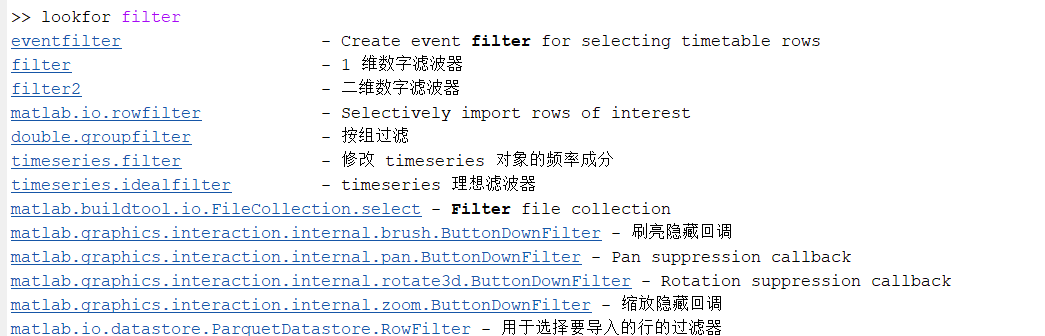
\includegraphics[width=0.8\linewidth]{lookfor_fliter.png}
    \caption{可用滤波器}
    \label{img:lookfor}
\end{figure}
\subsubsection{简单计算}
在Matlab 命令行中依次输入以下命令:
\begin{verbatim}
    pi*pi - 10 
    sin(pi/4) 
    ans ˆ 2 %<--- "ans" holds the last result 
    xx = sin( pi/5 ); 
    cos( pi/5 ) %<--- assigned to what? 
    yy = sqrt( 1 - xx*xx ) 
    ans
\end{verbatim}
部分结果展示如图\ref{img:var}所示,可见Matlab是类似于python那样动态性语言,一个表达式命令会将值
暂时赋给ans变量,自己也可以直接声明变量。
\begin{figure}[htbp]
    \centering
    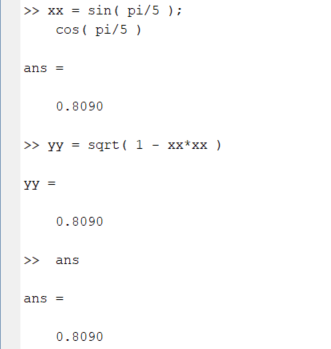
\includegraphics[width=0.6\linewidth]{var.png}
    \caption{实现简单计算}
    \label{img:var}
\end{figure}
\subsubsection{复数相关运算}
在Matlab 命令行中依次输入以下命令:
\begin{verbatim}
    real(zz), imag(zz)
    zz = 3 + 4i, ww =-3 + 4j
    abs([zz, ww]) %<-- Vector constructor
    conj(zz + ww)
    angle(zz)
    exp(j * pi)
    exp(j * [pi / 4, 0,-pi / 4 ])
\end{verbatim}
会得到相应的结果
\subsection{再识Matlab}
\subsubsection{Matlab数组索引}
\paragraph{冒号的含义}
在Matlab 命令行中依次输入以下命令:
\begin{verbatim}
    jkl = 2 : 4 : 17
    jkl = 0 : 6
    jkl = 99 :-1 : 88
    ttt = 2 : (1/9) : 4
    tpi = pi * [ 0:0.1:2 ]; %注意这里有分号
\end{verbatim}
所得结果如图\ref{img:colon}所示,可以了解到冒号的作用是“步进”,第一个数表示开始值,最后一个数表示结束值。如果存在中间值那么中间值为步距,不存在则默认步距为1。
\begin{figure}[htbp]
    \centering
    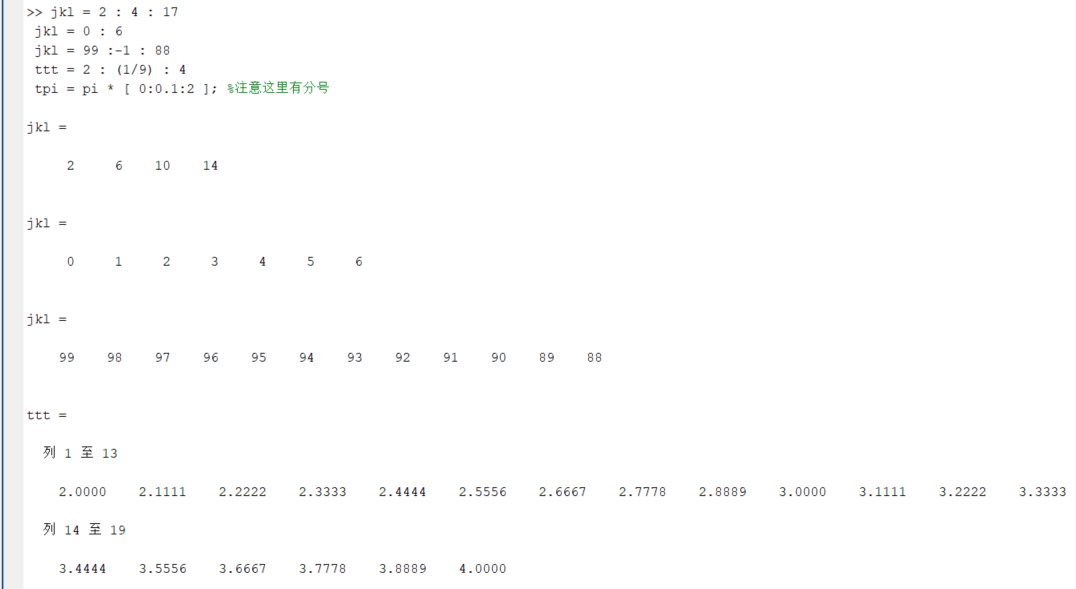
\includegraphics[width=0.7\linewidth]{colon.png}
    \caption{冒号相关命令}
    \label{img:colon}
\end{figure}
\paragraph{从向量中提取/插入数字}
在Matlab 命令行中依次输入以下命令:
\begin{verbatim}
    xx = [zeros(1,3), linspace(0,1,5), ones(1,4)]
    xx(4 : 6)
    size(xx)
    length(xx)
    xx(2 : 2 : length(xx))
    xx(2 : 2 : end)
\end{verbatim}
得到如图\ref{img:vector}所示的结果,可以知道:
第一行代码:创建了一个名为xx的数组,它是由三段拼接而成,第一段是由三个零组成的数组,第二段是从0到1均匀分布的包含5个元素的数组,最后一段由四个1组成的数组。它们由“[]”拼接成一个新的数组。

第二行代码:从xx中提取到位置4到6的元素生成一个新的数组。需要注意的是:Matlab中数组的索引是从1开始,而不是从0开始。

第三行代码:计算xx的大小,返回值是包含两个元素的数组,依次表示行数和列数,所以应该返回xx的行数:1,列数:12。

第四行代码:计算xx的长度,返回xx的长度:12。

最后后两行代码:类似于切片的操作,三个参数分别表示起点索引,步距和终点索引,返回一个新的数组。而end可以用来表示数组的末尾。
\begin{figure}[htbp]
    \centering
    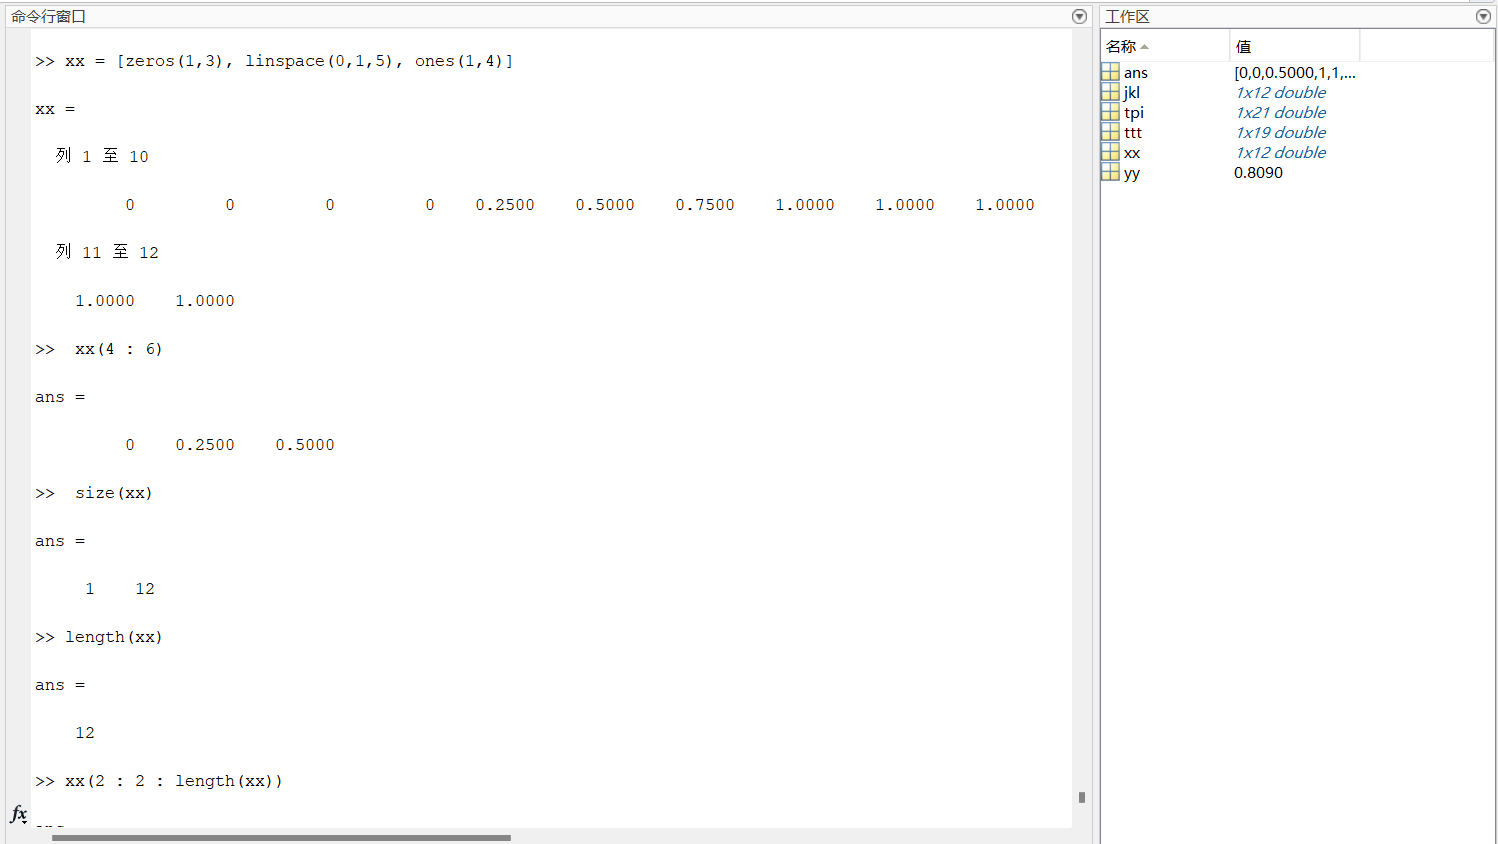
\includegraphics[width=0.7\linewidth]{vector.png}
    \caption{向量中提取或插入数字}
    \label{img:vector}
\end{figure}
\paragraph{修改向量中的值}
在Matlab的命令行中输入以下命令:
\begin{verbatim}
    yy = xx;
    yy(4:6) = pi*(1:3)
\end{verbatim}
可以知道数组可以直接赋给一个新的变量,可以使用类似与切片的写法批量修改数组中一段元素的值。
\begin{framed}
    现在写一条语句,xx用(b)中定义的方法,把xx的偶数索引的元素(即xx(2),xx(4)等)的值替换为常数$\pi^\pi$ 。使用向量替换,不要用循环。
\end{framed}
使用以下一行代码:
\begin{verbatim}
    xx(2 : 2 : end) = pi^pi
\end{verbatim}
如图\ref{img:even_substitution}所示,将xx的偶数索引的元素的值改成了常数$\pi^\pi$ 。
\begin{figure}[htbp]
    \centering
    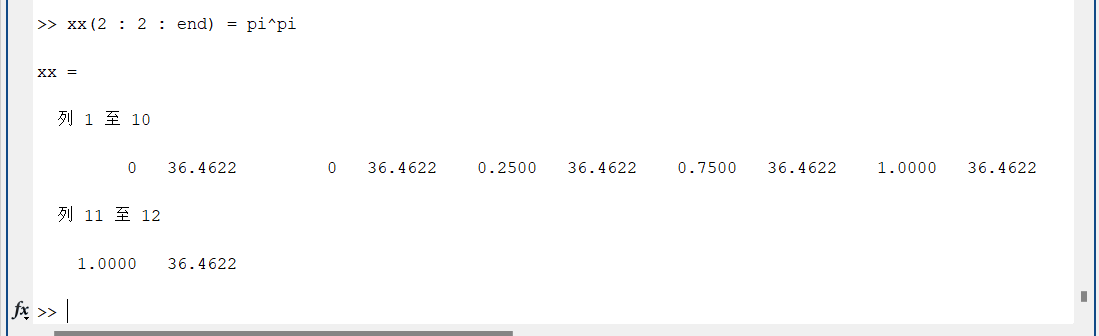
\includegraphics[width=0.7\linewidth]{even_substitution.png}
    \caption{替换向量索引为偶数的值}
    \label{img:even_substitution}
\end{figure}
\subsubsection{Matlab脚本文件}
\paragraph{关于向量的实验}
在Matlab的命令行中输入以下命令:
\begin{verbatim}
    xk = cos(pi * (0 : 11) / 4)
\end{verbatim}
得到如图\ref{img:vector_lab}所示的结果,该条命令是先经过(0:11)生成一个0到11的整数数组,然后再经过$pi * (0:11) / 4$将这些整数进行统一的计算生成一个全是弧度的12元素的数组,然后整个数组再进行余弦计算,得到最终的一个数组存在xk中。
xk(1)表示xk的第一个元素,没有xk(0),因为上文已经提到了数组的索引从1开始。
\begin{figure}[htbp]
    \centering
    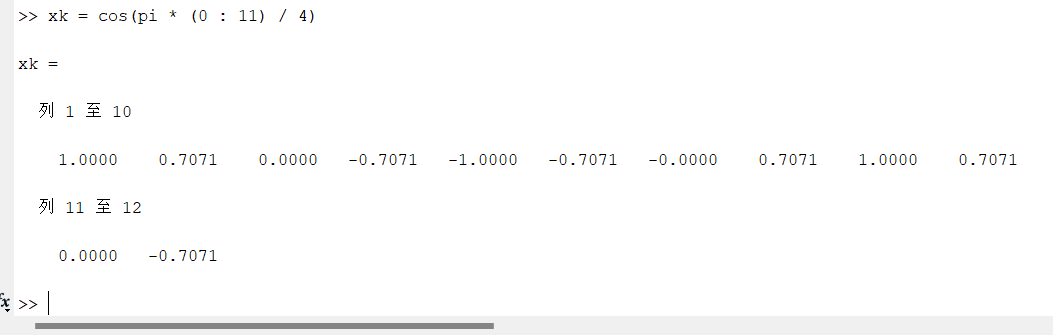
\includegraphics[width=0.7\linewidth]{vector_lab.png}
    \caption{关于向量的实验}
    \label{img:vector_lab}
\end{figure}
\paragraph{循环}
在Matlab的命令行中输入以下命令:
\begin{verbatim}
    yy = [ ]; %<--- initialize the yy vector to be empty 
    for k=-5:5 
    yy(k+6) = cos( k*pi/3 ) 
    end 
    yy 
\end{verbatim}
得到如图\ref{img:loop}所示的结果,向量yy被循环赋值
\begin{figure}[htbp]
    \centering
    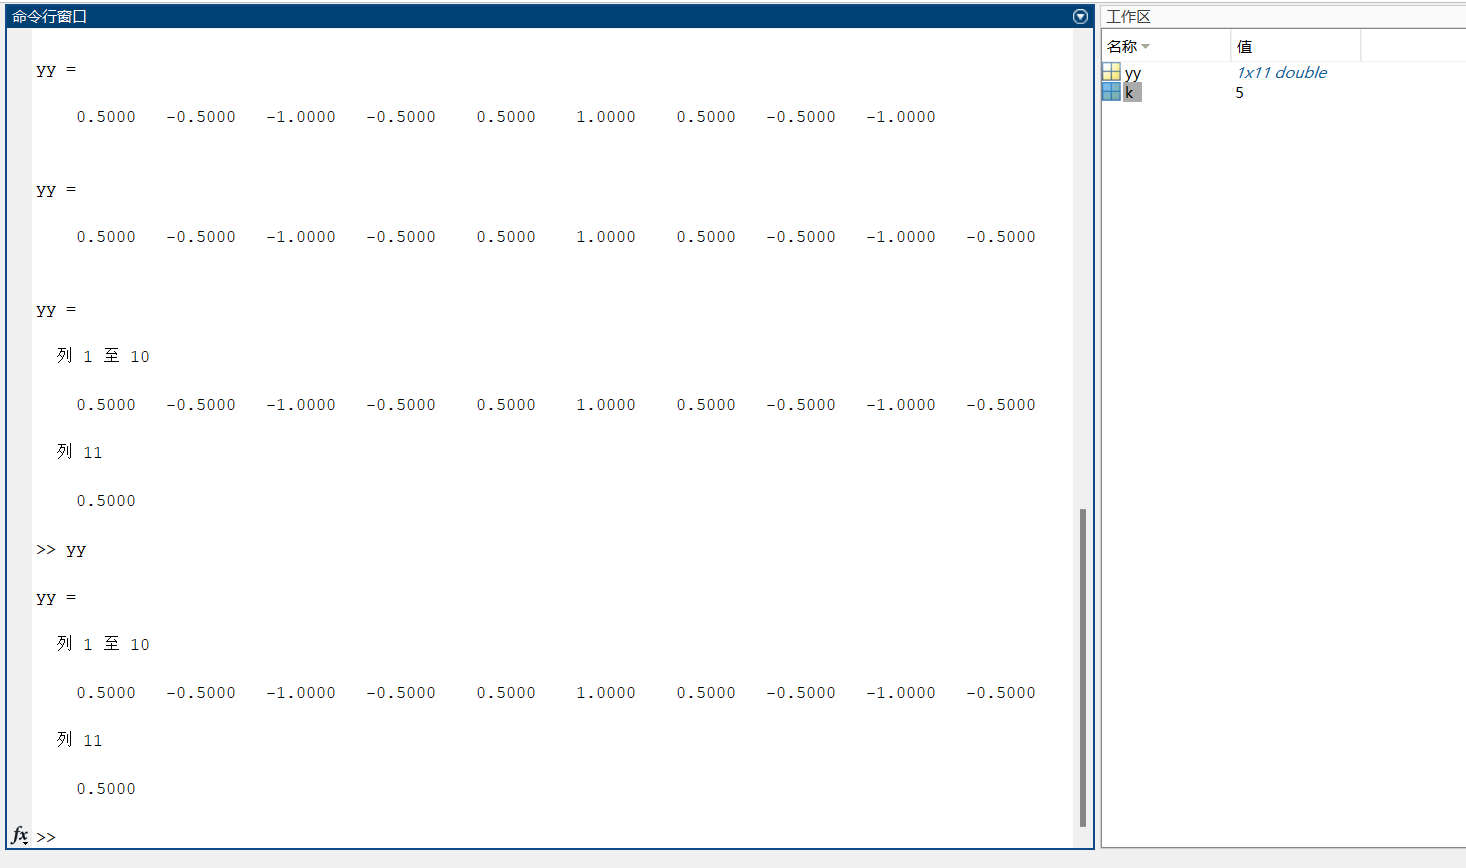
\includegraphics[width=0.7\linewidth]{loop.png}
    \caption{循环}
    \label{img:loop}
\end{figure}
\begin{framed}
    解释为什么需要写yy(k+6)。如果用yy(k)会发生什么?
\end{framed}
因为k从-5开始,而yy的索引必须从1开始,如果使用yy(k)将会报错。如果使用冒号而非循环,则应该是以下命令:
\begin{verbatim}
    yy = cos(pi * (-5:5) / 3)
\end{verbatim}
\paragraph{基本绘图命令}

在Matlab的命令行中输入以下命令:
\begin{verbatim}
    yy = xx.*xx- 3*xx;
    xx = [-3-1 0 1 3];
    plot(xx, yy)
    zz = xx + yy * sqrt(-1)
    plot(zz) %<---- complex values: plot imag vs. real
\end{verbatim}
得到如图\ref{img:plot}所示的结果,plot(xx,yy)命令和plot(zz)命令都是绘制一个以xx为横坐标,yy为纵坐标的图形,这里的zz是一个复数。
当xx是一个向量时:xx.*xx是将xx的所有元素都变为自身的平方。

当xx是一个矩阵时:xx.*xx时将xx的每一项变为本身的平方。
\begin{figure}[htbp]
    \centering
    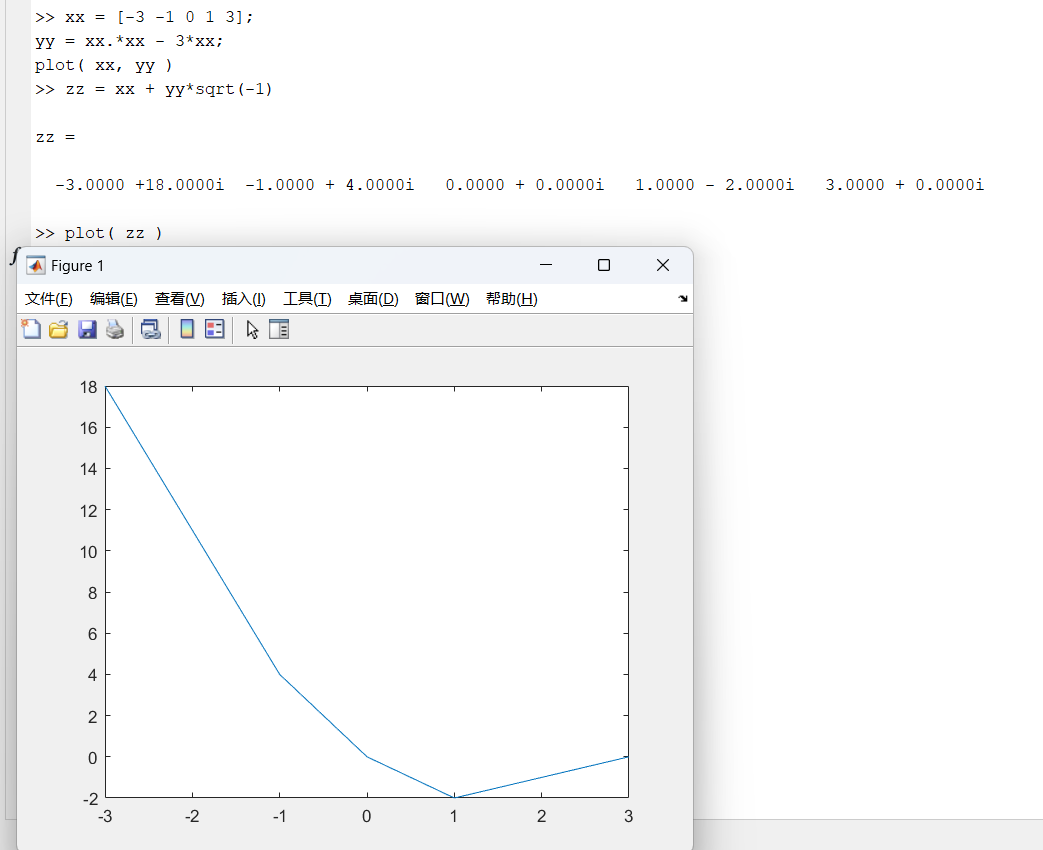
\includegraphics[width=0.7\linewidth]{plot.png}
    \caption{绘图命令结果}
    \label{img:plot}
\end{figure}

\paragraph{创建Matlab脚本文件}
创建一个名为mylab1.m的脚本文件,文件里是以下命令:
\begin{verbatim}
    clear all; close all;
    tt = -1 : 0.01 : 1; 
    xx = cos(5*pi*tt); 
    zz = 1.4*exp(j*pi/2)*exp(j*5*pi*tt); 
    plot(tt, xx, 'b-', tt, real(zz), 'r--') %<--- plot a sinusoid 
    grid on 
    title('TEST PLOT of a SINUSOID') 
    xlabel('TIME (sec)') 
\end{verbatim}
得到如图\ref{img:mylab1}所示的结果,红色虚线为zz的实部,蓝色实线为xx。
\begin{figure}[htbp]
    \centering
    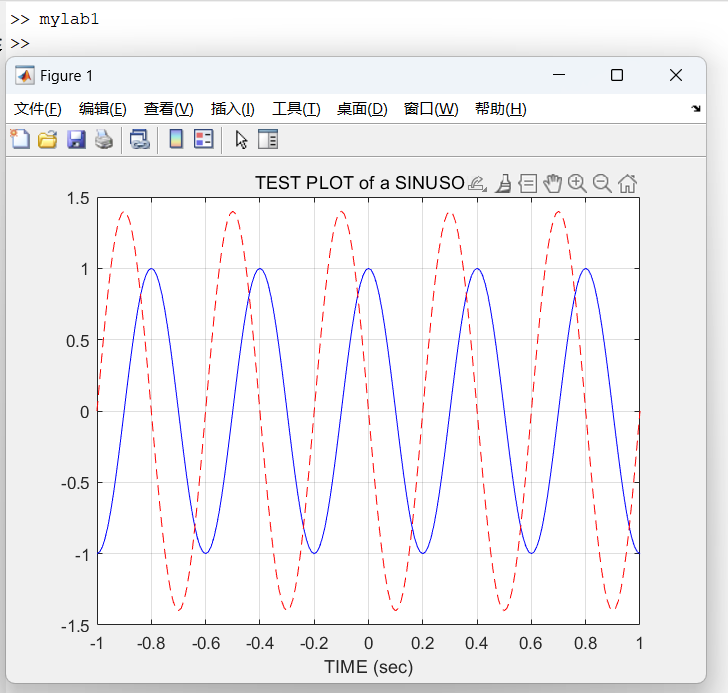
\includegraphics[width=0.7\linewidth]{mylab1.png}
    \caption{mylab1.m运行结果}
    \label{img:mylab1}
\end{figure}
\begin{framed}
    解释为什么real(zz)的图形是一个正弦曲线。它的相位和幅度是多少?由所绘图形的时移量计
    算相位。
\end{framed}
对zz = 1.4 * exp(j * pi / 2) * exp(j * 5 * pi * tt)命令进行计算:
$$
    zz = 1.4*e^\frac{j\pi}{2}*e^{j5\pi tt}=j*1.4*e^{j5\pi tt}=-1.4\sin(5\pi tt)+1.4j\cos(5\pi tt)
$$
所以$real(zz)=-1.4\sin(5\pi tt)$,即为一个正弦函数。
\subsubsection{Matlab与声音相关的函数命令}
要生成的正弦信号的频率为2000Hz,时长为0.9秒,采样率fs为11025个样本/秒。
采样率说明了采样点之间的时间间隔,所以时间向量应定义为:
$$
    tt=0:(1/fs):dur
$$
其中fs为采样率,dur为时长(以秒为单位)。那么就可以使用以下命令:
\begin{verbatim}
    fs = 11025;
    dur = 2;
    tt = (0 : 1 / fs : dur);
    xx = sin(2 * pi * 2000 * tt);
    plot(tt, xx);
    soundsc(xx, fs)
\end{verbatim}
得到如图\ref{img:sin_wave}所示绘制出来的波形,同时可以听到将近2秒的尖锐的声音
\begin{figure}[htbp]
    \centering
    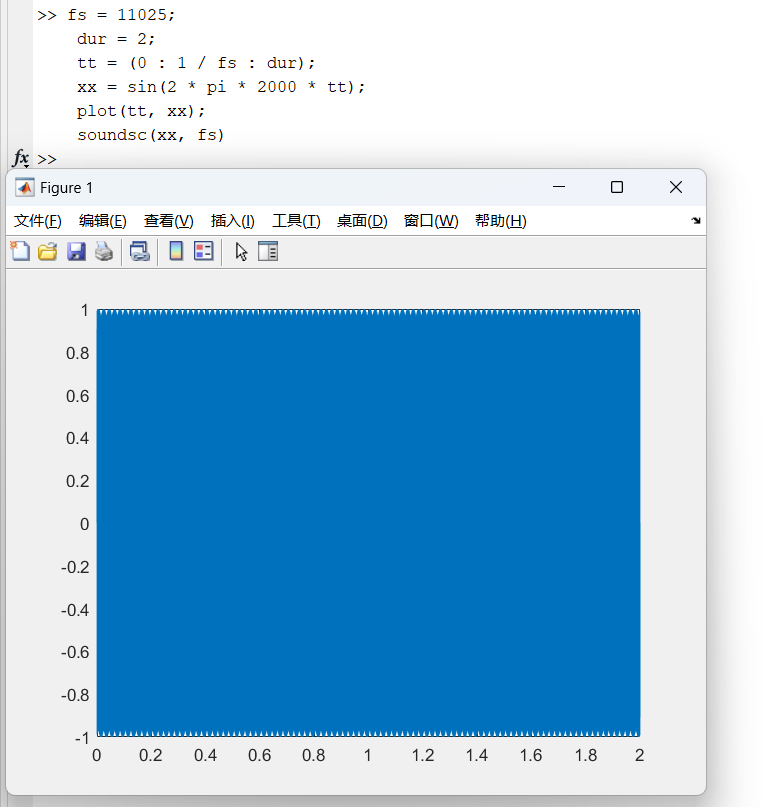
\includegraphics[width=0.6\linewidth]{sin_wave.png}
    \caption{正弦信号波形}
    \label{img:sin_wave}
\end{figure}

\subsection{用Matlab处理正弦信号}
\subsubsection{处理正弦信号}
\begin{framed}
    (a)生成一个时间向量tt,需要覆盖下面的(b)中频率为4000Hz的正弦信号的两个周期。tt的定义方式使用3.2(d)的方式。如果我们使用T表示正弦的周期,定义向量tt的开始时间为-T,结束时间为+T,那两个周期就会包括tt=0。最后,确保你们正弦波的每个周期有至少25个样本。也就是说,当你们使用冒号操作符定义时间变量时,要使增量足够小,才能保证每个周期可以产生至少25个样本。

    (b)生成以下两个4000Hz的正弦序列:$x_1(t)=A_1\cos(2\pi(4000)(t-t_{m1})),x_2(t)=A_2\cos(2\pi(4000)(t-t_{m2}))$。其中$A_1$是你的年龄,$A_2=1.2A_1$,$t_{m1} = (37.2/M)T$ ,$t_{m2} = -(41.3/D)T$ ,这里M和D分别是你生日的月和日,T是周期。

    (c)创建第3个正弦信号为 $x_3(t) = x_1(t) + x_2(t)$. 在Matlab中,这表示把两个正弦向量中的值对应相加。绘制$x_3(t)$在-T≤t≤T的图形,使用subplot(3,1,3)绘图。

    (d)对每个图都添加一个图名,图名都要包含你的姓名,用title函数。
\end{framed}
根据个人的情况可得:
$$A_1=19,A_2=1.2A_1=22.8$$
$$M=1,D=1$$
$$t_{m1}=(37.2/M)T=37.2T,t_{m2}=-(41.3/D)T=-41.3T$$
所以在脚本文件$processing_sinusoid_signals.m$中输入以下代码:
\begin{verbatim}
    f = 4000; %frequency 4000Hz
    T = 1 / f; %cycle 1/4000
    fs = 30;
    %Sampling frequency 30 per sec
    tt = (-1 * T) : (1 / (fs * f)) : T;
    A1 = 19;
    A2 = 1.2 * A1;
    M = 1;
    D = 1;
    tm1 = (37.2 / M) * T;
    tm2 =-(41.3 / D) * T;
    x1t = A1 * cos(2 * pi * 4000 * (tt- tm1));
    x2t = A2 * cos(2 * pi * 4000 * (tt- tm2));
    x3t = x1t + x2t;
    subplot(3,1,1);
    plot(tt,x1t);
    title('赵展 x1(t)');
    subplot(3,1,2);
    plot(tt,x2t);
    title('赵展 x2(t)');
    subplot(3,1,3);
    plot(tt,x3t);
    title('赵展 x3(t)')
\end{verbatim}
得到如图\ref{img:processing_sinusoidal_signals}所示绘制出来的波形。
\begin{figure}[htbp]
    \centering
    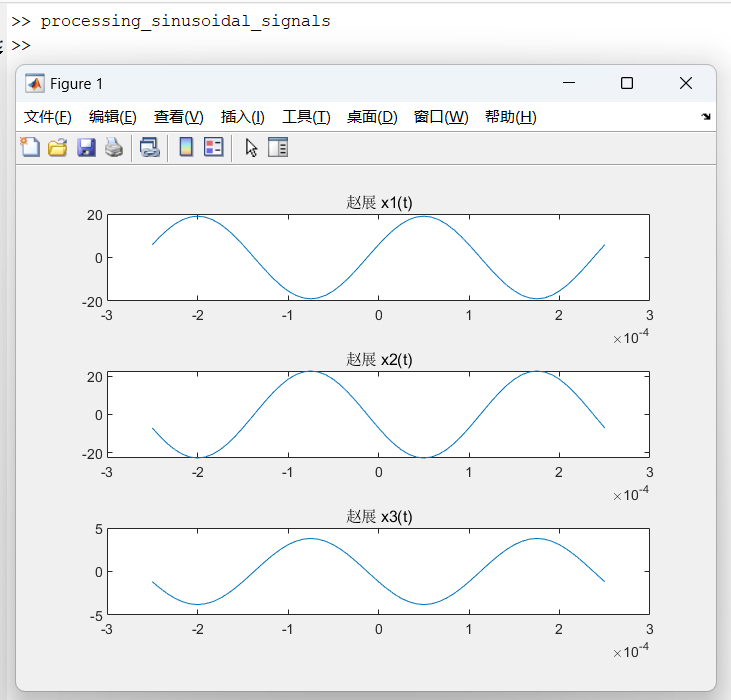
\includegraphics[width=0.7\linewidth]{processing_sinusoidal_signals.png}
    \caption{处理正弦信号波形图}
    \label{img:processing_sinusoidal_signals}
\end{figure}
\subsubsection{复数幅度}
\begin{framed}
    用一条语句生成以上正弦信号$x_1(t)$ 的值,可以使用复数幅度表示方法:$x_1(t) = Re\{Xe^{jt}\}$,其中X和w为某个常数。
\end{framed}
已知$x_1(t)=A_1\cos(2\pi(4000)(t-37.2T))$,所以可以将$x_1(t)$写成:$Re\{19e^{j2\pi{4000t-37.2}}\}$,在Matlab的命令行中输入以下命令:
\begin{verbatim}
    f = 4000; %frequency 4000Hz
    T = 1 / f; %cycle 1/4000
    fs = 30;
    %Sampling frequency 30 per sec
    tt = (-1 * T) : (1 / (fs * f)) : T;
    x1 = real(19 * exp(j * 2 * pi * (4000 * tt- 37.2 )));
    plot(tt, x1)
\end{verbatim}
得到如图\ref{img:complex_amplitude}所示绘制出来的波形,和上边使用正弦函数表达式画出来的x1t图一样
\begin{figure}[htbp]
    \centering
    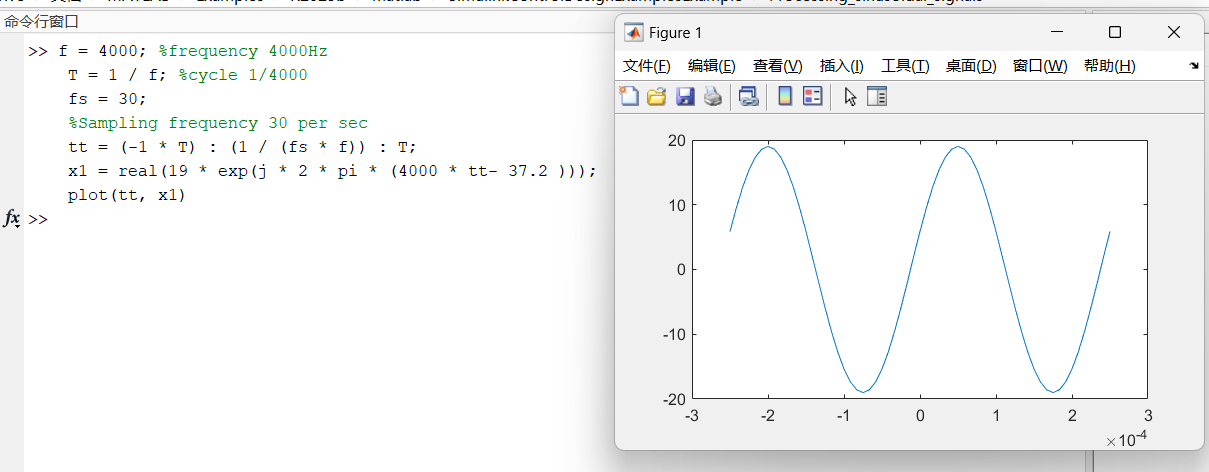
\includegraphics[width=0.7\linewidth]{complex_amplitude.png}
    \caption{复数幅度表示正弦函数}
    \label{img:complex_amplitude}
\end{figure}
\subsection{复指数简介}
\subsubsection{向量化}
\begin{framed}
    用这种向量化的方法编写2-3行代码完成以下Matlab代码,不使用循环。(注:当xx是向量时,xx*xx和xx.*xx是不同的)
    \begin{verbatim}
        %--- make a plot of a weird signal 
        N = 200; 
        for k=1:N 
        xk(k) = k/50; 
        rk(k) = sqrt( xk(k)*xk(k) + 2.25 ); 
        sig(k) = exp(j*2*pi*rk(k)); 
        end 
        plot( xk, real(sig), 'mo-' ) 
    \end{verbatim}
\end{framed}
使用向量化方法就是将循环等繁冗的代码转化成冒号形式,转化后的代码如下:
\begin{verbatim}
    xk = (1 : 200) / 50;
    sig = exp(j * 2 * pi * sqrt(xk .* xk + 2.25));
    plot (xk, real(sig), 'mo-')
\end{verbatim}
在Matlab中运行之后得到如图\ref{img:vector_transform}所示的结果。
\begin{figure}[htbp]
    \centering
    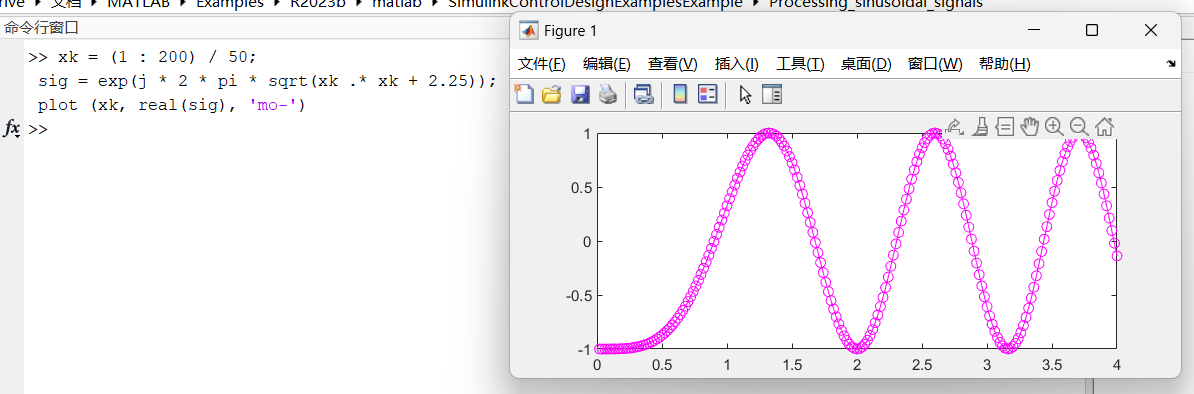
\includegraphics[width=0.7\linewidth]{vector_transform.png}
    \caption{向量化之后代码运行结果}
    \label{img:vector_transform}
\end{figure}
\subsubsection{函数}
在Matlab中新建一个脚本文件$testcos.m$用来写一个函数,正确写法如下:
\begin{verbatim}
    function [xx,tt] = goodcos(ff,dur) 
    tt = 0:1/(100*ff):dur; %-- gives 100 samples per period 
    xx = cos(2*pi*ff*tt)
\end{verbatim}
在命令行中输入:testcos(1,10)后显示出如图\ref{img:testcos}所示的结果(部分),表明函数调用成功。
如果输入:goodcos(1,10)则会报错:"函数或变量 'goodcos' 无法识别"。
需要注意的是调用和函数是用的脚本文件名称而非脚本文件中写的函数的名称,但是最好这两个名称保持一致。
\begin{figure}[htbp]
    \centering
    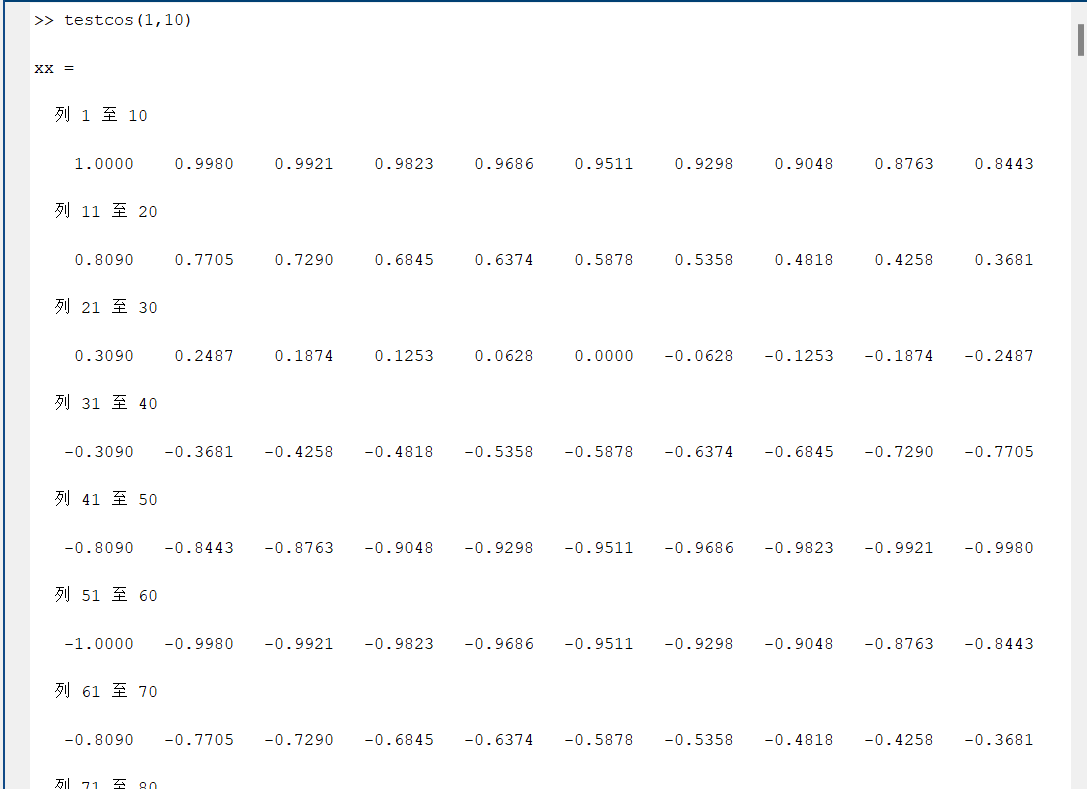
\includegraphics[width=0.7\linewidth]{testcos.png}
    \caption{测试函数运行结果}
    \label{img:testcos}
\end{figure}

\subsection{复指数}
\subsubsection{生成正弦信号的M-文件}
\begin{framed}
    写一个可以生成单一正弦信号x(t) = Acos(ωt+φ)的函数,使用4个输入参量:幅度A,频率,相位和时长dur。函数应当返回两个输出参量:正弦信号的值x和对应的时间t。
    确保函数生成的正弦信号在每个周期有20个值,函数名为$one\_cos()$。
    提示:可借鉴上面的goodcos()函数。

    绘制你们的$one\_cos()$函数,参数选为:A=95,$\omega =200\pi$弧度/秒,$\phi =\frac{\pi}{5} $弧度,时长为0.025秒。
    推导所绘图形的周期和相位是否正确。
    如果周期以毫秒为单位是多少?
\end{framed}
根据要求新建一个脚本文件$one\_cos.m$,其中内容如下:
\begin{verbatim}
    function [x, t] = one_cos(A, Ang_freq, phase, dur)
    t = 0 : 1 / (20 * (Ang_freq / 2 / pi)) : dur;
    x = A * cos(Ang_freq * t + phase)
\end{verbatim}
保存之后在命令行中调用:
\begin{verbatim}
    [xx, tt] = one_cos(95, 200 * pi, pi / 5, 0.025);
    plot(tt, xx)
\end{verbatim}
得到的如图\ref{img:one_cos}所示的结果,生成正弦函数的表达式应为$x(t)=95\cos(200\pi t+\frac{\pi}{5})$,角频率为$200\pi$可以算出频率$f=\frac{\omega}{2\pi}=100$,周期$T=\frac{1}{f}=\frac{1}{100}s=10ms$。
从周期上看,0.025s绘制出2.5个周期,从相位上看,初相位$\phi=\frac{\pi}{5}$对应到图像中$95\cos(\frac{\pi}{5})\approx 76.9$,
可以看出图像确为该函数。
\begin{figure}[htbp]
    \centering
    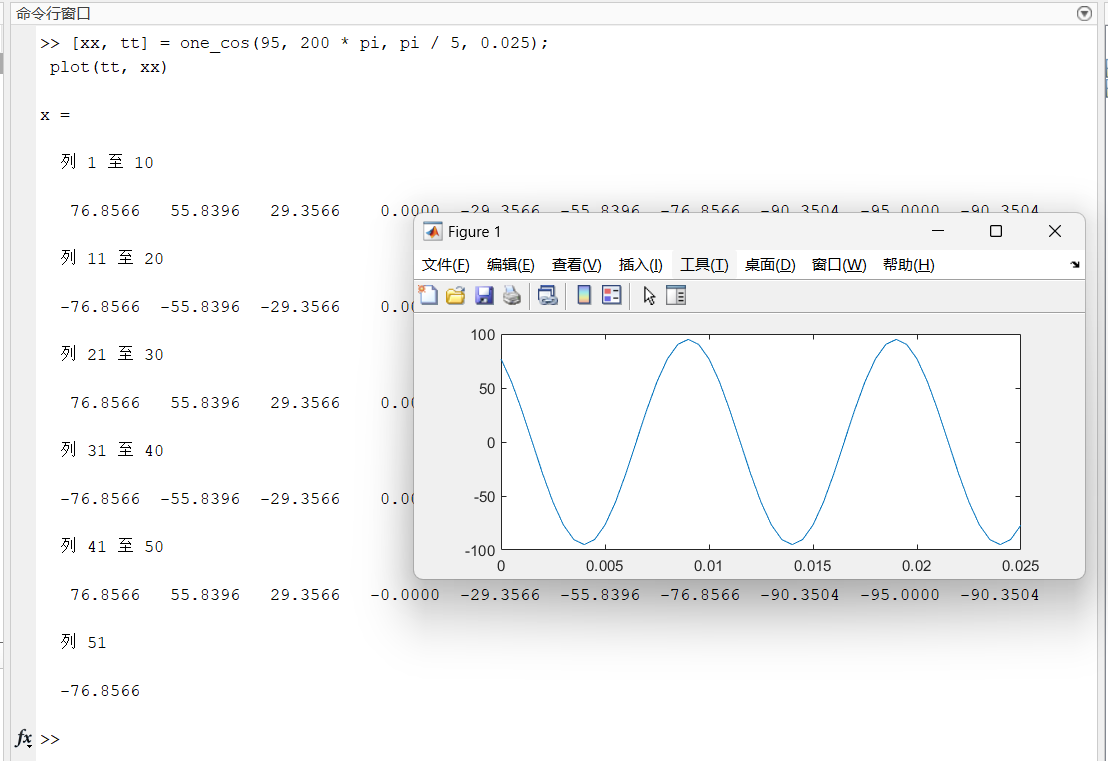
\includegraphics[width=0.7\linewidth]{one_cos.png}
    \caption{$one\_cos$生成正弦函数的图像}
    \label{img:one_cos}
\end{figure}

\subsection{线性调频脉冲chrip}
\subsubsection{chirp 信号的Matlab合成方法}
在Matlab的命令行中输入以下命令生成一个chirp信号:
\begin{verbatim}
    fsamp = 11025;
    dt = 1 / fsamp;
    dur = 1.8;
    tt = 0 : dt : dur;
    psi = 2 * pi * (100 + 200 * tt + 500 * tt .* tt);
    xx = real(7.7 * exp(j * psi));
    soundsc(xx, fsamp)
\end{verbatim}
\begin{framed}
    (a)确定合成信号的总时长(秒),确定tt向量的长度(样本数)

    (b)在Matlab中,只能合成离散时间信号,所以对于chirp信号,我们处理为:
    $$x(t_n)=Acos(2\pi \mu t_n^2+2\pi f_0t_n+\phi )$$
    其中,$t_n=nT_s$表示离散时间值。在以上的Matlab代码中,$t_n$的值是多少?A, $\mu$, $f_0$和$\phi$的值是多少?

    (c)确定以上Matlab代码合成的频率的范围(Hz为单位)。手绘瞬时频率随时间的变化情况。听到的最小频率和最大频率是多少?

    (d)听听信号的频率是上升还是下降(使用soundsc())。注意soundsc()需要知道信号创建时的采样率。详见帮助。
\end{framed}
上述命令运行之后我可以听到一个音调由低到高的声音,合成信号的总时长为1.8s,tt向量的长度(样本数)为19846。
上述代码中生成的chirp信号可以处理为:
$$
    x(t_n)=7.7cos(2\pi \times 500tt^2+2\pi \times 200tt + 200\pi)
$$
其中$t_n=nT_s$,$t_n$即为tt,$T_s=dt=\frac{1}{fsamp}=\frac{1}{11025}$,$A=7.7,\mu=500,f_0=200,\phi=200\pi$。
tt = 0 时,频率为200Hz,tt=1.8时,频率为200+2*500*1.8=2000Hz,可以绘制图像如图\ref{img:freq_time}所示。
\begin{figure}[htbp]
    \centering
    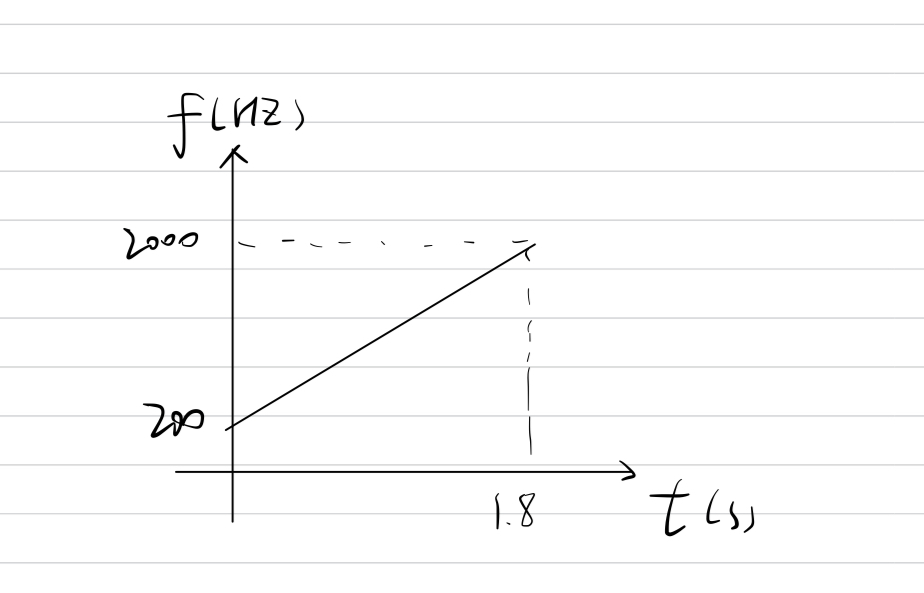
\includegraphics[width=0.7\linewidth]{freq_time.png}
    \caption{f关于t的图像}
    \label{img:freq_time}
\end{figure}

\subsubsection{chirp的函数}
\begin{framed}
    请生成一个chirp,其频率起始于2500Hz,终止于500Hz。时长应当为1.5秒。听听你的chirp。
\end{framed}
在Matlab中新建一个脚本文件mychirp.m,输入以下内容:
\begin{verbatim}
    function [xx, tt] = mychirp(f1, f2, dur, fsamp)
    if(nargin < 4)
        fsamp = 11025;
    end
    tt = 0 : 1 / (fsamp) : dur;
    psi = 2 * pi * (f1 * tt + (f2- f1) / dur / 2 * tt .* tt);
    xx = real(exp(j * psi))
\end{verbatim}
在Matlab中输入以下命令进行调用:
\begin{verbatim}
    [xx, tt] = mychirp(2500, 500, 1.5, 11025);
    soundsc(xx,11025)
\end{verbatim}
最终可以听到音调逐渐降低的声音,持续1.5秒。

\subsubsection{声谱图}
为了了解声谱图,在Matlab中输入以下命令:
\begin{verbatim}
    fs=8000;
    xx = cos(3000 * pi * (0: 1 / fs : 0.5));
    specgram(xx, 1024, fs)
\end{verbatim}
可以得到如图\ref{img:sonagraph}所示的声谱图。
\begin{figure}[htbp]
    \centering
    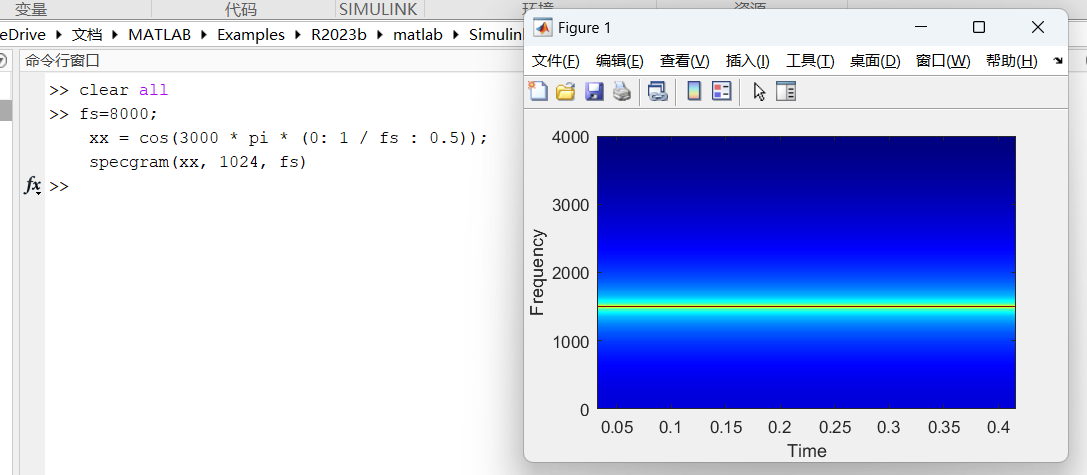
\includegraphics[width=0.7\linewidth]{sonagraph.png}
    \caption{声谱图}
    \label{img:sonagraph}
\end{figure}

\subsubsection{chirp的声谱图}
在Matlab中输入以下命令调用mychirp生成chirp信号并查看其声谱图:
\begin{verbatim}
    [xx, tt] = mychirp(5000, 300, 3, 11025);
    soundsc(xx, 11025);
    specgram(xx, 2048, 11025)
\end{verbatim}
可以听到音调逐渐降低的声音,生成的声谱图如图\ref{img:chirp_sonagraph}所示。
\begin{figure}[htbp]
    \centering
    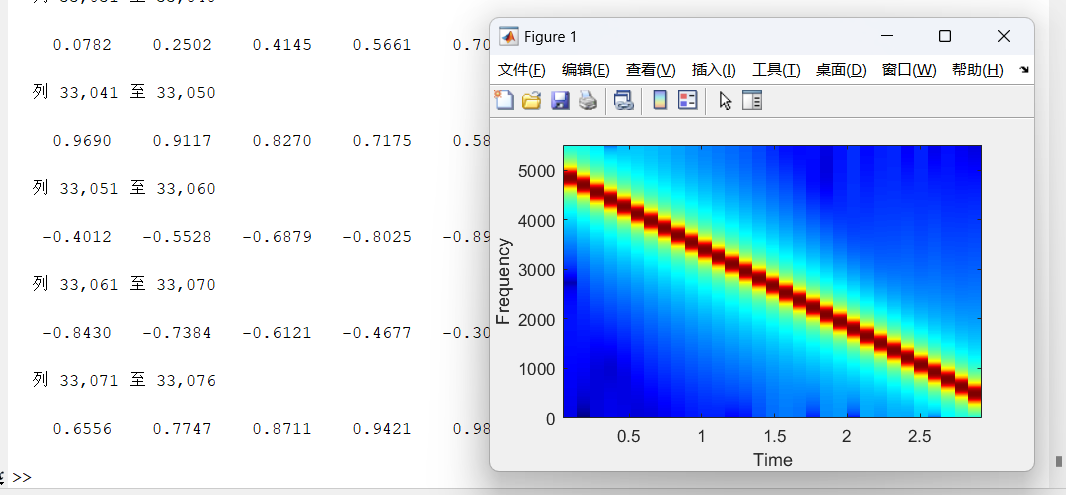
\includegraphics[width=0.7\linewidth]{chirp_sonagraph.png}
    \caption{chirp的声谱图}
    \label{img:chirp_sonagraph}
\end{figure}

\subsubsection{有趣的chirp}
\begin{framed}
    再合成一个chirp信号,使用如下参数:

    1.总时长为3秒,采样率为fs=11025Hz

    2.频率起始于3000Hz,终止于-2000Hz(负频率)

    听一听信号。频率是怎么变化的?
    显示这个chirp信号的声谱图。
    使用频谱理论(正频率成分和负频率成分)解释你听到的声音和看到的声谱图。
\end{framed}
在Matlab中输入以下命令合成一个新的chirp信号:
\begin{verbatim}
    [xx, tt] = mychirp(3000,-2000, 3, 11025);
    soundsc(xx, 11025);
    specgram(xx, 2048, 11025);
\end{verbatim}
可以听到一个音调逐渐降低又升高的声音,说明频率先降低后升高,而得到声谱图如图\ref{img:interesting_chirp_sonagraph}所示也是如此。
声谱图中频率逐渐降低又升高,这是因为频率变为负的时候,只是相当于角频率的方向发生了改变,而真正的听到的频率还是增加的。
\begin{figure}[htbp]
    \centering
    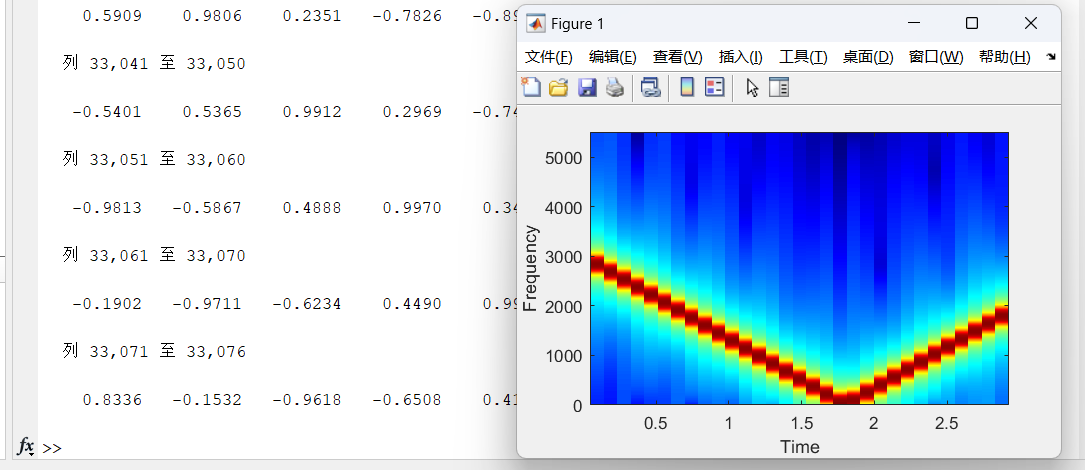
\includegraphics[width=0.7\linewidth]{interesting_chirp_sonagraph.png}
    \caption{有趣的chirp的声谱图}
    \label{img:interesting_chirp_sonagraph}
\end{figure}
\section{实验小结}
通过本次实验,我成功熟悉了Matlab的一些基本使用,因为是从软件学院转到了这里,第一次接触Matlab,所以此次实验花了我不少的时间和精力。
同时经老师推荐,这也是我第一次使用\LaTeX 进行排版设计,掌握了一些基本的排版、公式代码。
所以这次实验对我来说收获满满。希望可以给后续的实验和课程打下一个好的基础。
\end{document}